\documentclass[10pt]{beamer}
\usepackage[orientation=landscape,size=custom,width=16,height=9,scale=0.5,debug]{beamerposter}
\usepackage[french]{babel}
\usepackage[OT1]{fontenc}
\usepackage{textcomp}
\usepackage{csquotes}
\usepackage{dirtytalk}
\usepackage{float}
\usepackage{framed}
\usepackage{listings}
\usepackage{adjustbox}
\usepackage{array}
\usepackage{epstopdf}
\usetheme[progressbar=frametitle,numbering=fraction]{metropolis}
\usepackage{appendixnumberbeamer}
\newcommand{\ousommesnous}{Où sommes-nous ?}
\usepackage{hyperref}
\hypersetup{
    colorlinks = true,
    anchorcolor = .,
    linkcolor = .,
    urlcolor = blue,
}
\usepackage{booktabs}
\usepackage[scale=2]{ccicons}
\usepackage{pgfplots}
\usepgfplotslibrary{dateplot}

\usepackage{xspace}
\newcommand{\themename}{\textbf{\textsc{metropolis}}\xspace}

\newcommand{\tocsss}{\begin{frame}[allowframebreaks]{Table des matières de la sous-section : \subsecname}
    \tableofcontents[
    currentsection,
    currentsubsection,
    hideothersubsections,
    sectionstyle=hide/hide
]
\end{frame}}


\newcommand{\tocss}{
    \begin{frame}[allowframebreaks]{Table des matières de la section : \secname}
    \tableofcontents[
        currentsection,
        currentsubsection,
        hideothersubsections,
        sectionstyle=show/hide,
    ]
\end{frame}}

\usepackage{color}
\lstloadlanguages{C,C++,csh,Java}

\definecolor{red}{rgb}{0.6,0,0} 
\definecolor{blue}{rgb}{0,0,0.6}
\definecolor{green}{rgb}{0,0.8,0}
\definecolor{cyan}{rgb}{0.0,0.6,0.6}

\lstset{
language=csh,
basicstyle=\tiny\ttfamily,
numbers=left,
numberstyle=\tiny,
numbersep=5pt,
tabsize=2,
extendedchars=true,
breaklines=true,
frame=b,
stringstyle=\color{blue}\ttfamily,
showspaces=false,
showtabs=false,
xleftmargin=17pt,
framexleftmargin=17pt,
framexrightmargin=5pt,
framexbottommargin=4pt,
commentstyle=\color{green},
morecomment=[l]{//}, %use comment-line-style!
morecomment=[s]{/*}{*/}, %for multiline comments
showstringspaces=false,
morekeywords={ abstract, event, new, struct,
as, explicit, null, switch,
base, extern, object, this,
bool, false, operator, throw,
break, finally, out, true,
byte, fixed, override, try,
case, float, params, typeof,
catch, for, private, uint,
char, foreach, protected, ulong,
checked, goto, public, unchecked,
class, if, readonly, unsafe,
const, implicit, ref, ushort,
continue, in, return, using,
decimal, int, sbyte, virtual,
default, interface, sealed, volatile,
delegate, internal, short, void,
do, is, sizeof, while,
double, lock, stackalloc,
else, long, static,
enum, namespace, string},
keywordstyle=\color{cyan},
identifierstyle=\color{red}
}

\definecolor{main}{RGB}{35,54,59}
\usepackage{caption}
\DeclareCaptionFont{white}{\color{white}}
\DeclareCaptionFormat{listing}{\colorbox{main}{\parbox{\textwidth}{\hspace{15pt}#1#2#3}}}
\captionsetup[lstlisting]{format=listing,labelfont=white,textfont=white, singlelinecheck=false, margin=0pt, font={bf,footnotesize}}

\setbeamertemplate{frame footer}{\insertsectionhead}

\title{Systèmes de Gestion de Bases de Données — 2e}
\subtitle{Chapitre 1 : Concepts de base}
\date{\today}
\author{Daniel Schreurs}
\institute{Haute École de Province de Liège}
%\titlegraphic{\hfill\includegraphics[height=1.5cm]{logo.eps}}

\begin{document}

\maketitle

\setbeamerfont{subsection in toc}{size=\small}
\setbeamerfont{subsubsection in toc}{size=\normalsize}
\setbeamertemplate{section in toc}[sections numbered]
\setbeamertemplate{subsection in toc}[subsections numbered]
\setbeamertemplate{subsubsection in toc}[subsubsections numbered]
\begin{frame}[allowframebreaks]{Table des matières du chapitre}
    \tableofcontents[subsectionstyle=show/show/hide,subsubsectionstyle=show/show/hide,]
\end{frame}

\section{Base de données}
\begin{frame}{Table des matières de la section}
    \setbeamertemplate{section in toc}[sections numbered]
    \setbeamertemplate{subsection in toc}[subsections numbered]
    \tableofcontents[currentsection,currentsubsection,
        hideothersubsections,
        sectionstyle=show/shaded,
    ]
\end{frame}

\subsection{BD et SGBD}
\begin{frame}{\secname : \subsecname}
    \begin{itemize}
        \item \emph{BD} : collection de données concernant un sujet enregistrées sur un support permanent accessible par l’ordinateur.
        \item \emph{SGBD} : logiciel qui permet à un utilisateur d’exploiter une BD
    \end{itemize}
\end{frame}

\subsection{Propriétés}
\tocsss

\subsubsection{Être un ensemble organisé/structuré}
\begin{frame}{\subsecname : \subsubsecname}
    Stocker les données de manière à ce que leur exploitation soit efficace !
    L’organisation doit tenir compte du mode d’accès le plus courant aux données.
    Exemple :
    Catalogue d’une bibliothèque : lecture principalement
    Fichier des prêts : lecture et écriture
    \begin{enumerate}
        \item Catalogue d’une bibliothèque : lecture principalement
        \item Fichier des prêts : lecture et écriture
    \end{enumerate}
\end{frame}


\subsubsection{Être un ensemble intégré}
\begin{frame}{\subsecname : \subsubsecname}
    Exemple : chaque service de la bibliothèque accède aux mêmes données centralisées.
    \begin{figure}[H]
        \begin{center}
            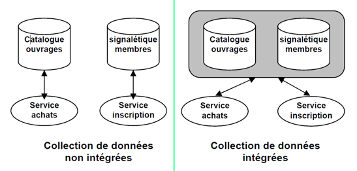
\includegraphics[width=0.5\textwidth]{../assets/img/etre_un_ensemble_integre.png}
            \caption{Exemple d'une gestion intégrée}
            \label{Fig:new-etre_un_ensemble_integre}
        \end{center}
    \end{figure}
\end{frame}

\subsubsection{Correspondre fidèlement à la réalité}
\begin{frame}{\subsecname : \subsubsecname}
    \begin{itemize}
        \item Pour forcer les données à rester fidèles à la réalité, on définit, des contraintes d’intégrité sur la BD.
        \item Ces contraintes d’intégrité sont la traduction informatique des règles de fonctionnement.
        \item On ne stocke pas que des données, mais on stocke aussi des contraintes portant sur ces données.
    \end{itemize}
\end{frame}

\subsubsection{Contenir les données opérationnelles sur un sujet donné}
\begin{frame}{\subsecname : \subsubsecname}
    \begin{itemize}
        \item Les membres et les ouvrages sont appelés \emph{entités} dans le jargon des bases de données. Les entités sont stockées dans la base de données. Un emprunt associe un membre et un ouvrage : un emprunt est une association. Les associations sont aussi stockées dans la base de données.
        \item Les entités et les associations sont appelées données opérationnelles.
    \end{itemize}
\end{frame}
\subsubsection{Être multi-utilisateurs}
\begin{frame}{\subsecname : \subsubsecname}
    \begin{itemize}
        \item Les données doivent être accessibles en même temps par plusieurs utilisateurs.
              Chaque utilisateur doit avoir l’impression qu’il est seul à utiliser la base.
        \item Le partage simultané des données implique l’existence de mécanismes de protections : confidentialité, gestions des accès concurrents, sauvegarde, reprise après panne.
    \end{itemize}
\end{frame}

\subsubsection{Être non-redondante}
\begin{frame}{\subsecname : \subsubsecname}
    \begin{itemize}
        \item La non-redondance implique que chaque donnée ne soit stockée qu’une seule fois dans la base.  Elle assure la cohérence. De plus, elle permet d’économiser la place disque.
        \item La redondance contrôlée peut être utilisée pour satisfaire à des besoins de vitesse de traitements et de ce fait, gagner en temps de réponse.
        \item Des trigger (déclencheurs) seront utilisés pour éviter les incohérences
    \end{itemize}
\end{frame}


\section{Système de gestion de base de données}
\tocss

\subsection{Les Fonctions}
\tocsss


\subsubsection{Description et définition}
\begin{frame}{\subsecname : \subsubsecname}
    Le concepteur ou administrateur de la base doit pouvoir :
    \begin{itemize}
        \item Créer la base de données;
        \item Définir ses paramètres physiques;
        \item Définir les objets qu’elle contient.
    \end{itemize}
\end{frame}

\subsubsection{Manipulation}
\begin{frame}{\subsecname : \subsubsecname}
    \label{manipulation}
    La manipulation des données est un terme générique pour désigner :
    \begin{itemize}
        \item La \emph{recherche} d’information;
        \item L'\emph{ajout};
        \item La \emph{modification};
        \item La \emph{suppression} de données.
    \end{itemize}
\end{frame}

\subsubsection{Intégrité}
\begin{frame}{\subsecname : \subsubsecname}
    Le SGBD doit :
    \begin{itemize}
        \item Permettre de définir des règles d’intégrité \footnote{représentant les règles de gestion du système informatisé}.
        \item Il doit aussi assurer qu’à tout moment\footnote{Au moins avant et après chaque transaction.}, les valeurs présentes dans la base ou qu’un utilisateur tente d’introduire respectent ces contraintes.
    \end{itemize}
\end{frame}

\subsubsection{Confidentialité}
\begin{frame}{\subsecname : \subsubsecname}
    La fonction de confidentialité permet :
    \begin{itemize}
        \item D’assurer que chaque utilisateur n’effectue que les manipulations\footnote{Tel que défini au slide \ref{manipulation}.} autorisées sur certaines données.
    \end{itemize}
\end{frame}


\subsubsection{Concurrence d’accès}
\begin{frame}{\subsecname : \subsubsecname}
    \begin{itemize}
        \item Les accès concurrents \footnote{Quand des utilisateurs différents tentent d’accéder en même temps aux mêmes données.} doivent pouvoir être traités. Sinon, ils peuvent introduire des incohérences dans la base de données !
    \end{itemize}
\end{frame}

\begin{frame}{\subsecname : Mais aussi}
    Cette liste de fonctions n’est pas exhaustive. On peut aussi évoquer :
    \begin{itemize}
        \item La reprise après panne;
        \item Précompilateur;
        \item Optimiseur;
        \item Journalisation;
        \item Gérer les accès concurrents;
        \item Gérer le "cache";
        \item Gérer les sauvegardes;
        \item Gérer l'espace disque, les index, etc.
    \end{itemize}
\end{frame}

\subsection{Architecture d’un SGBD}
\begin{frame}{\secname : \subsecname}
    En général, les SGBD relationnels sont constitués de deux parties
    \begin{figure}
        \begin{center}
            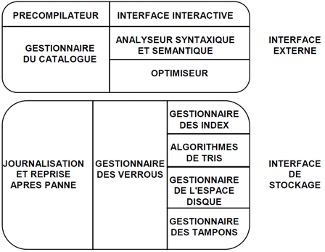
\includegraphics[width=0.4\textwidth]{../assets/img/architecture_sgbd.jpg}
            \caption{Architecture d’un SGBD}
            \label{Fig:architecturesgbd}
        \end{center}
    \end{figure}
\end{frame}

\begin{frame}{\secname : \subsecname}
    \begin{alertblock}{Important}
        Le \emph{Catalogue} ou \emph{Méta base} ou \emph{Dictionnaire} ou \emph{Tables Sytèmes}
        \begin{itemize}
            \item Est mis à jour automatiquement par le SGBD
            \item Constitue une mini base de données contenant des informations sur la BD
            \item Est stocké dans la BD elle-même et peut être interrogé comme les données de la BD elle-même
            \item Contient la description de tous les objets présents dans la base : tables, domaines, contraintes, privilèges, fichiers, index, procédures stockées, déclencheurs, vues, objets, …
            \item Il NE s’agit PAS d’un fichier spécial en dehors de la base
        \end{itemize}
    \end{alertblock}
\end{frame}

\begin{frame}{\secname : \subsecname}
    \begin{columns}
        \column{0.6\textwidth}
        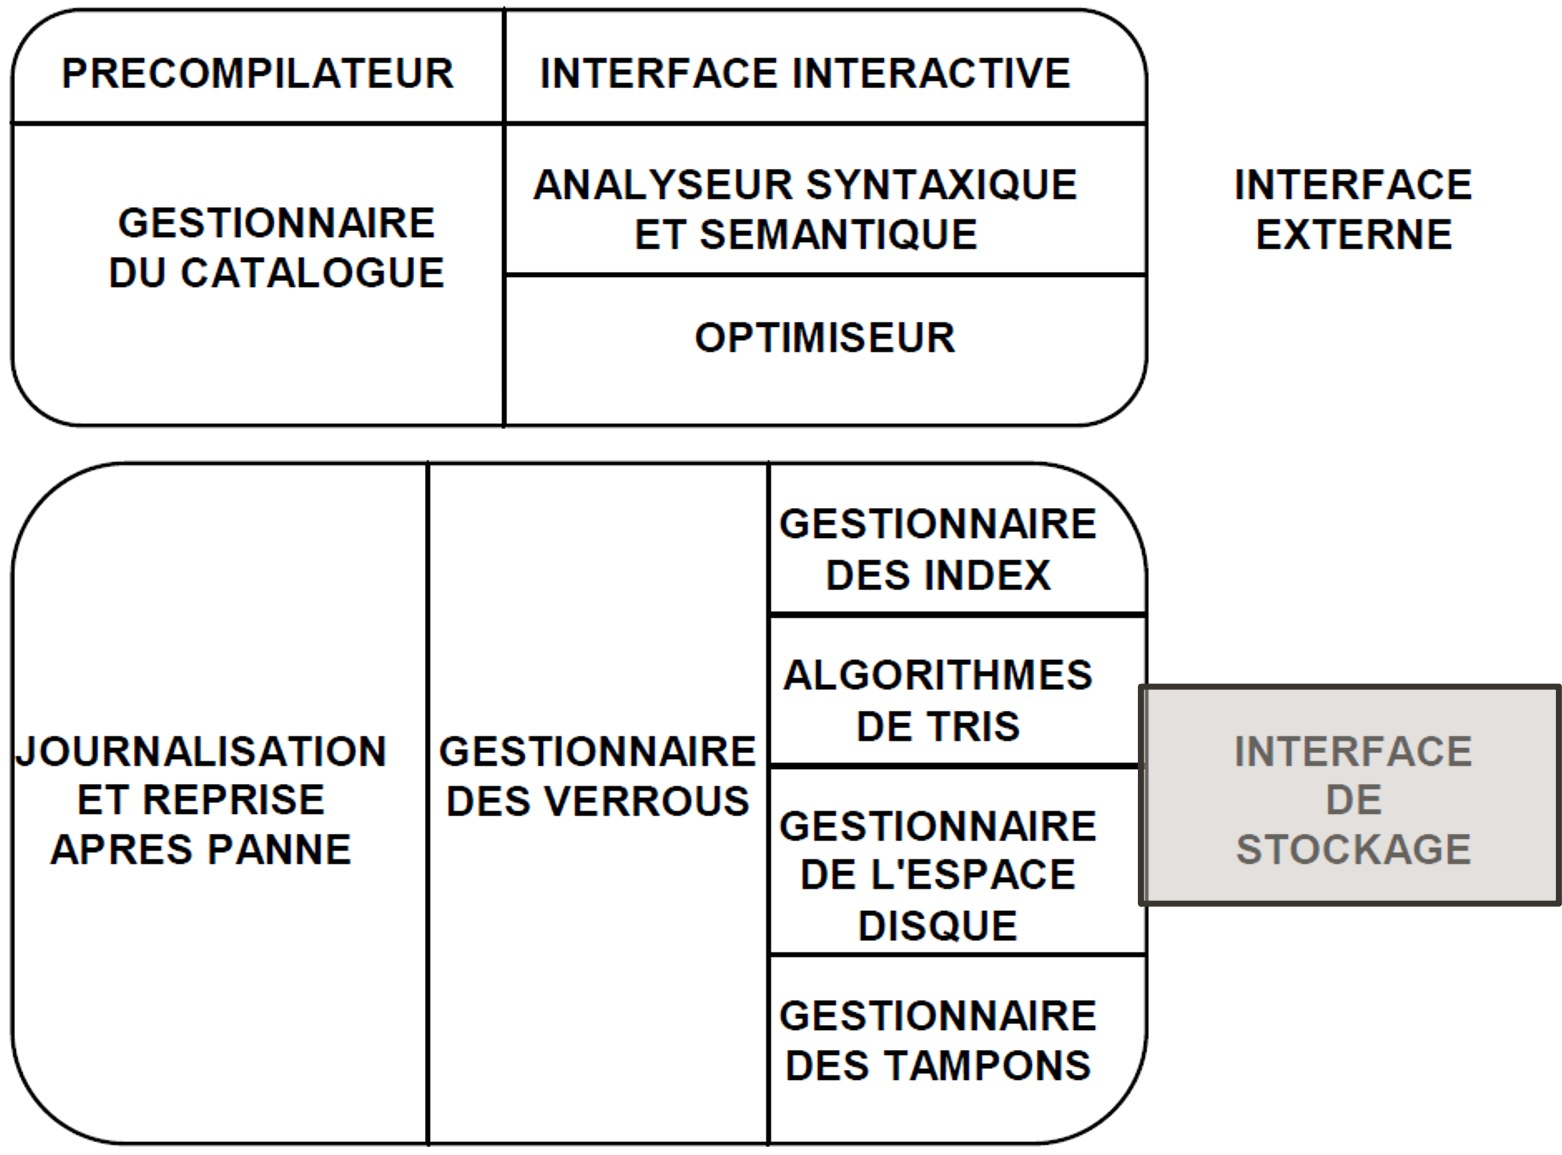
\includegraphics[width=0.8\linewidth]{../assets/img/architecture_sgbd--3.jpg}
        \column{0.4\textwidth}
        L’interface de stockage s’occupe de tout ce qui concerne l’accès aux données stockées sur disques
    \end{columns}
\end{frame}

\begin{frame}{\secname : \subsecname}
    \begin{columns}
        \column{0.6\textwidth}
        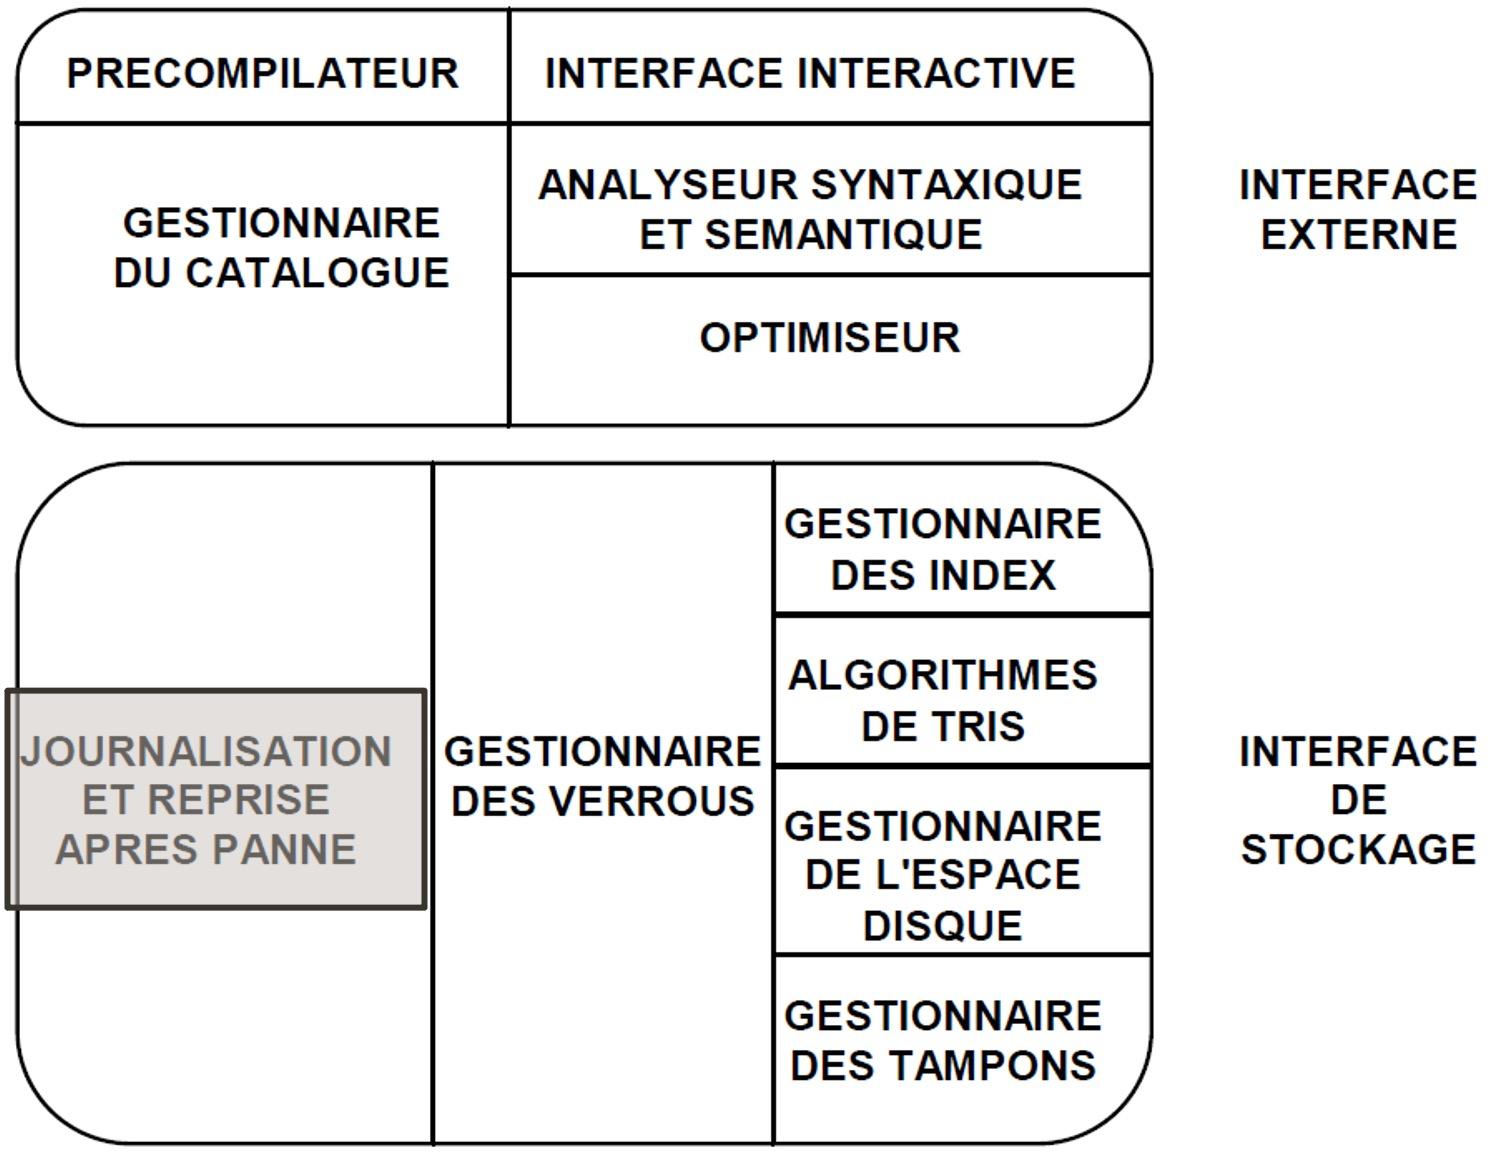
\includegraphics[width=0.8\linewidth]{../assets/img/architecture_sgbd--4.jpg}
        \column{0.4\textwidth}
        \begin{itemize}
            \item La journalisation et reprise après pannes assure la fonction de sécurité de fonctionnement.
            \item Nous ne l’aborderons pas cette année.
        \end{itemize}
    \end{columns}
\end{frame}

\begin{frame}{\secname : \subsecname}
    \begin{columns}
        \column{0.6\textwidth}
        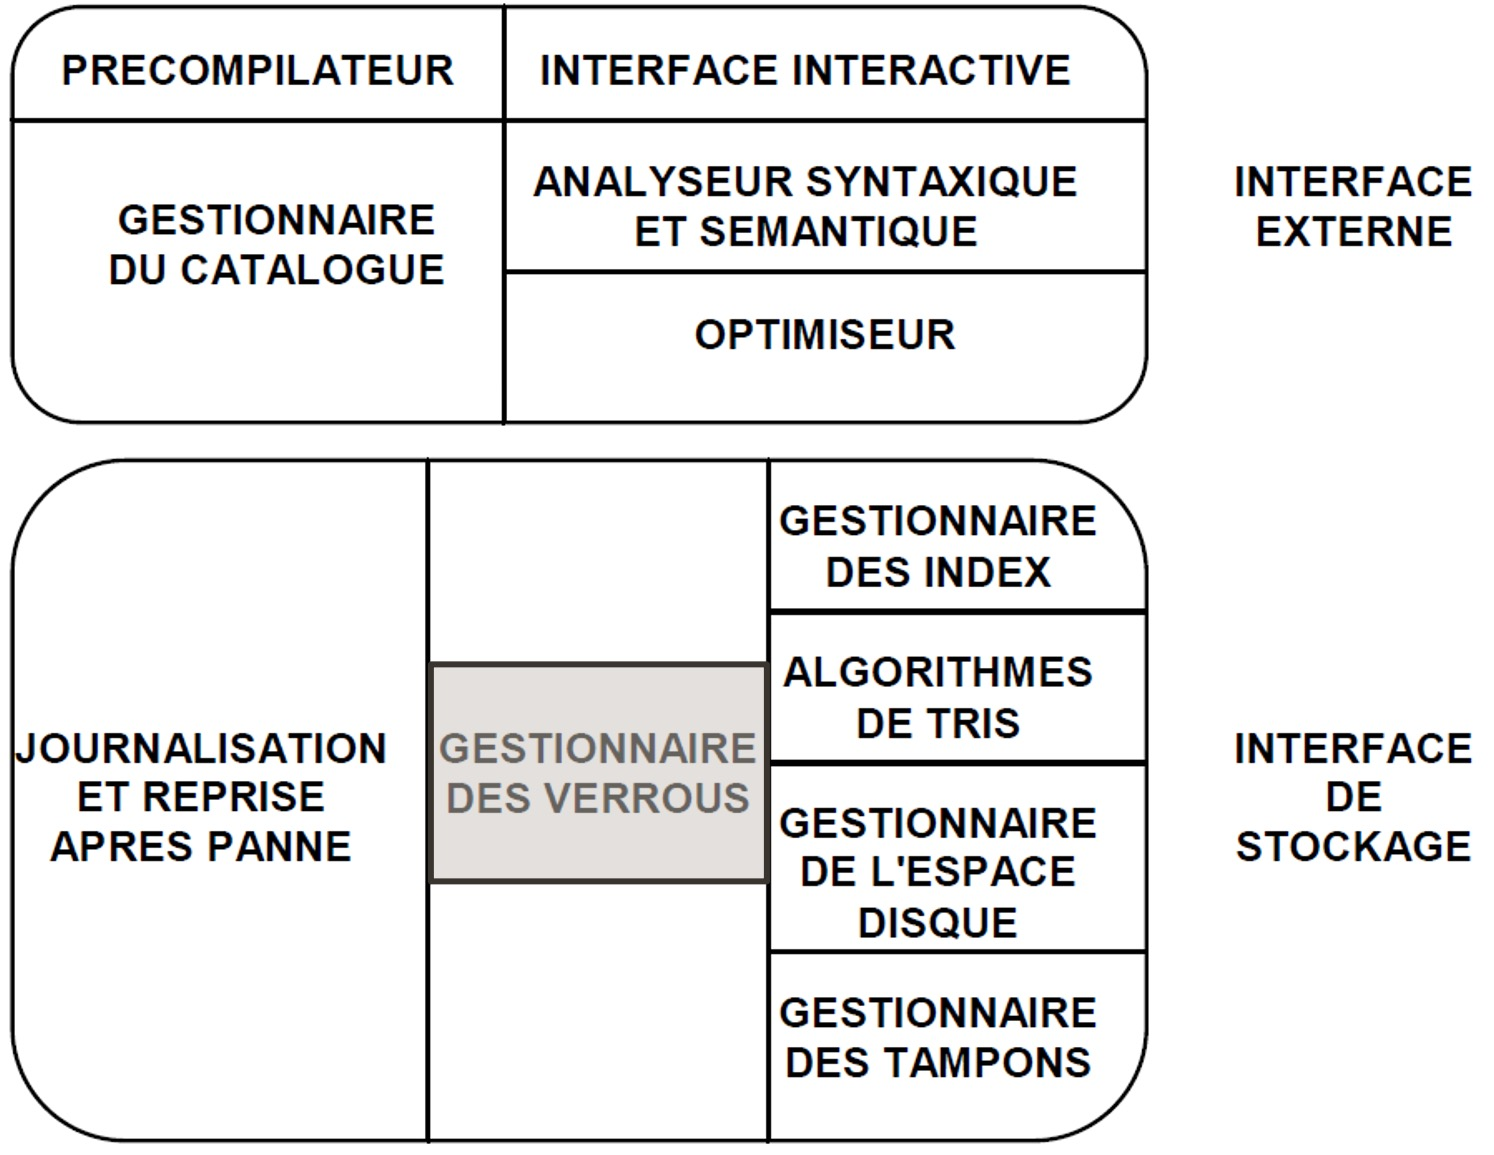
\includegraphics[width=0.8\linewidth]{../assets/img/architecture_sgbd--5.jpg}
        \column{0.4\textwidth}
        \begin{itemize}
            \item Le gestionnaire des verrous assure la fonction de concurrence d’accès.
            \item Les 4 gestionnaires restants servent à minimiser le nombre d’entrées/sorties, l’espace mémoire alloué sur disque, etc.
        \end{itemize}
    \end{columns}
\end{frame}

\section{Indépendance données}
\subsection{Programmes}
\tocsss
\begin{frame}{\secname : \subsecname}
    \metroset{block=fill}
    \begin{alertblock}{Important}
        Il est important de pouvoir changer la structure logique ou physique d’une base sans devoir changer les programmes d’applications qui l’utilisent.
    \end{alertblock}
    Exemple :

    \begin{itemize}
        \item On ajoute de nouvelles entités ou associations;
        \item On décompose une entité en sous-entités.
    \end{itemize}
\end{frame}


\subsubsection{L’approche traditionnelle par les fichiers}
\begin{frame}{\subsecname : \subsubsecname}
    \begin{figure}
        \begin{center}
            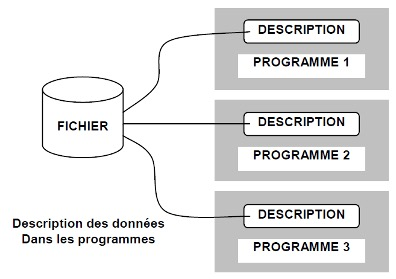
\includegraphics[width=0.5\textwidth]{../assets/img/par_fichier.jpg}
            \caption{L’approche traditionnelle par les fichiers}
            \label{Fig:par_fichier}
        \end{center}
    \end{figure}
\end{frame}



\begin{frame}{\subsecname : \subsubsecname}
    \begin{itemize}
        \item Les données contenues dans les fichiers sont directement associées aux programmes par une description contenue dans le programme lui-même.
        \item Dans chaque programme utilisant le fichier, on aura une déclaration du type (structure par exemple) permettant la manipulation des données du fichier.
        \item Aucune indépendance possible entre les données et les programmes.
    \end{itemize}
\end{frame}

\subsubsection{Organisation autour d’une base de données}
\begin{frame}{\subsecname : \subsubsecname}
    \begin{figure}
        \begin{center}
            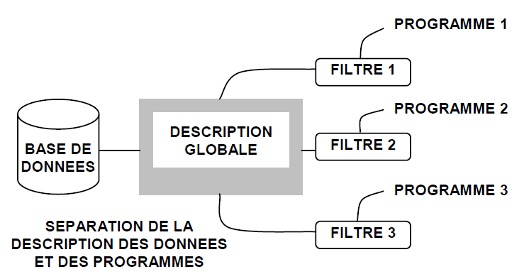
\includegraphics[width=0.55\textwidth]{../assets/img/par_sgbd.jpg}
            \caption{Organisation autour d’une base de données}
            \label{Fig:par_sgbd}
        \end{center}
    \end{figure}
\end{frame}

\begin{frame}{\subsecname : \subsubsecname}
    \begin{itemize}
        \item La description des informations est centralisée;
        \item Chaque programme utilise un filtre pour désigner les informations qu’il utilise.
    \end{itemize}
\end{frame}

\begin{frame}{\subsecname : \subsubsecname}
    Objectifs fondamentaux d’un système base de données :
    \begin{itemize}
        \item L’indépendance des données par rapport aux programmes de traitements
        \item La prise en compte des associations entre les différentes données
        \item Le partage simultané des données entre plusieurs utilisateurs
    \end{itemize}
\end{frame}

\subsubsection{Indépendance des données et des programmes}

\begin{frame}{\subsecname : \subsubsecname}
    \begin{figure}
        \begin{center}
            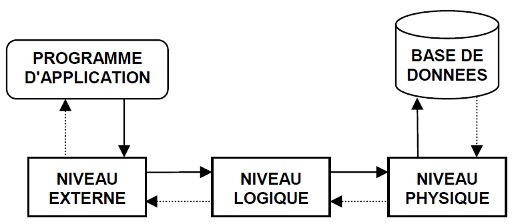
\includegraphics[width=0.55\textwidth]{../assets/img/par_sgbd_et_programme.jpg}
            \caption{Indépendance des données et des programmes}
            \label{Fig:par_sgbd_et_programme}
        \end{center}
    \end{figure}
\end{frame}

\begin{frame}{\subsecname : \subsubsecname}
    \begin{figure}
        \begin{center}
            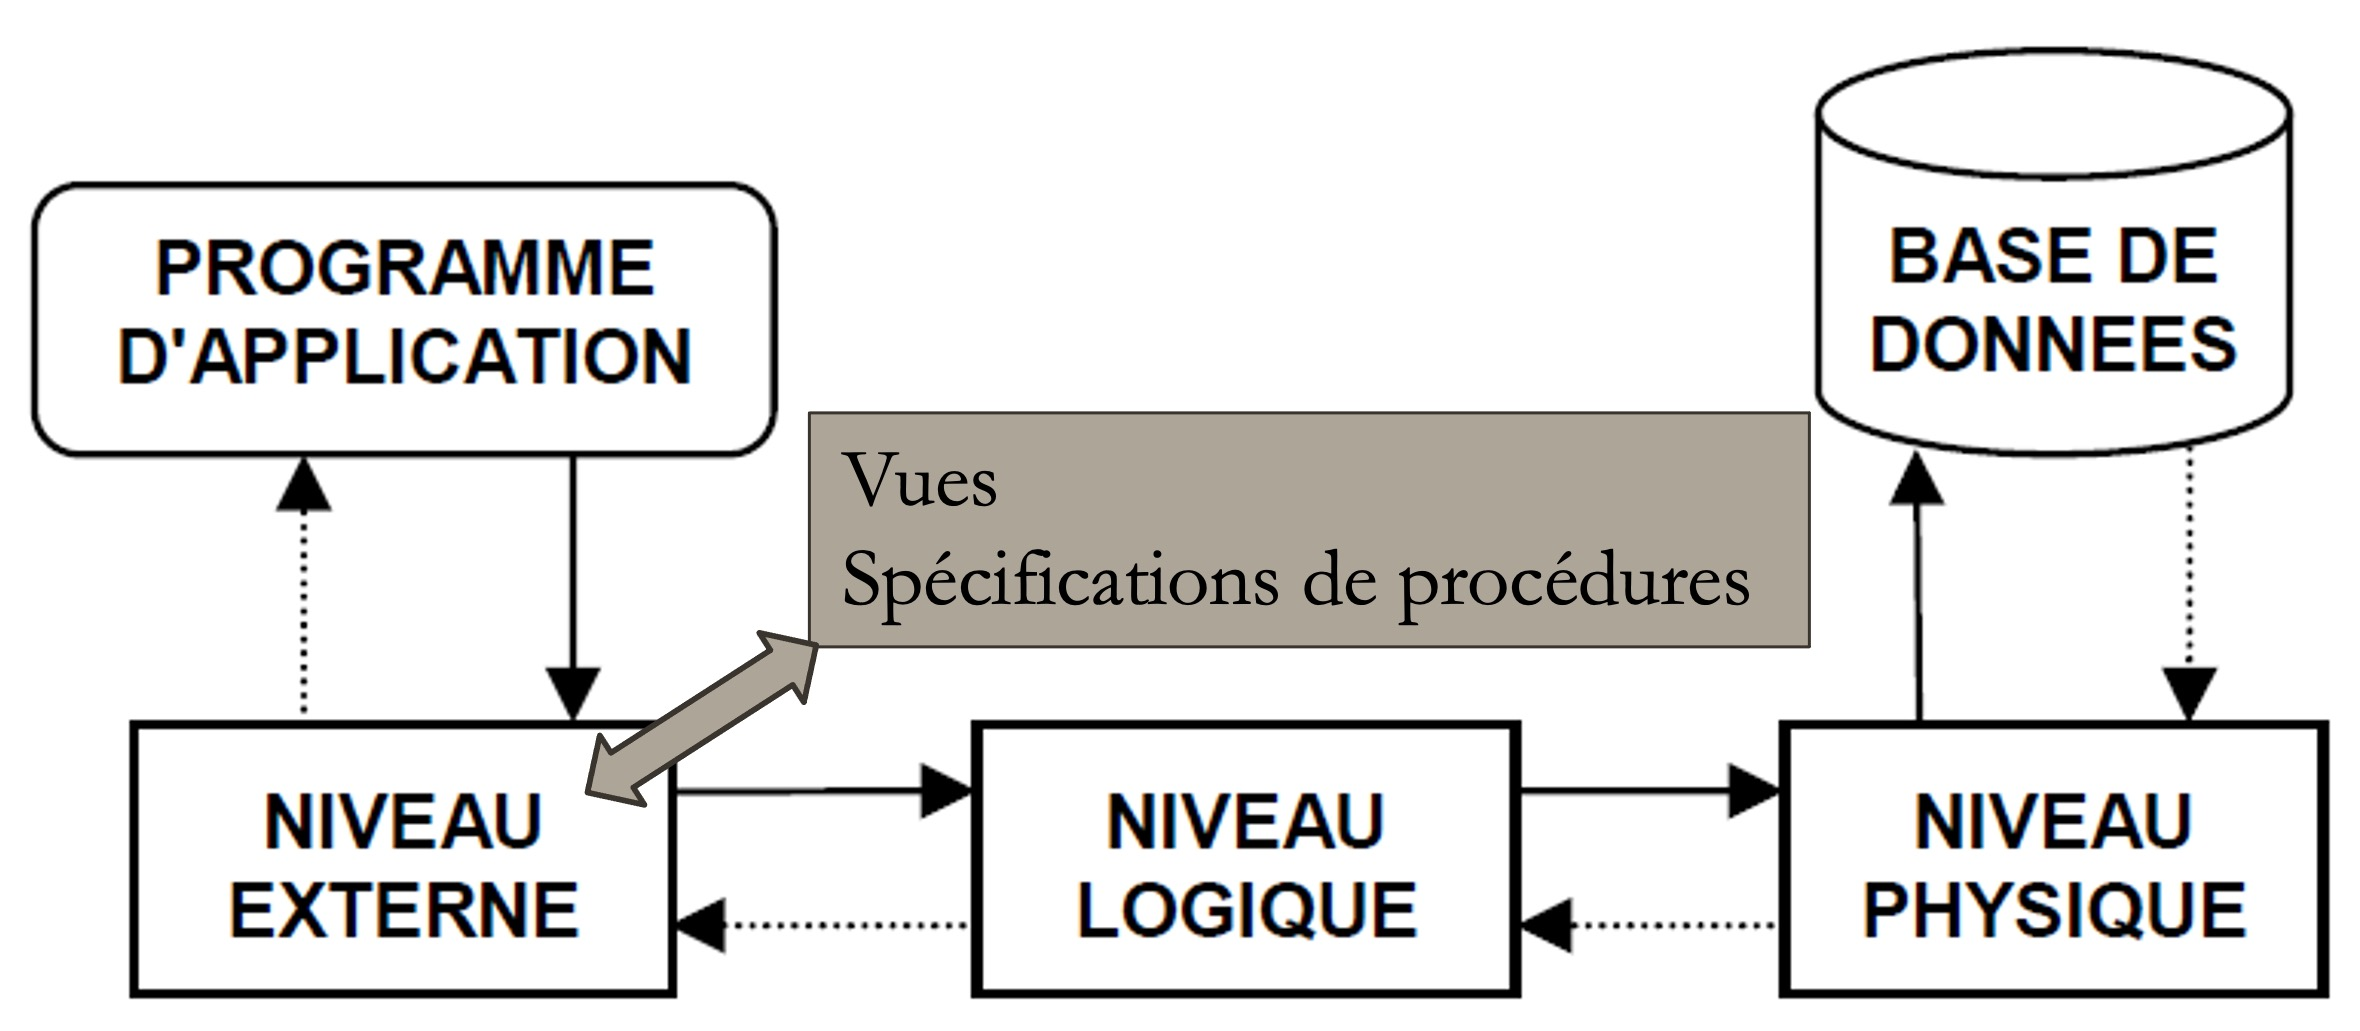
\includegraphics[width=0.55\textwidth]{../assets/img/par_sgbd_et_programme--1.jpg}
            \caption{Indépendance des données et des programmes}
            \label{Fig:par_sgbd_et_programme--1}
        \end{center}
    \end{figure}
\end{frame}

\begin{frame}{\subsecname : \subsubsecname}
    \begin{figure}
        \begin{center}
            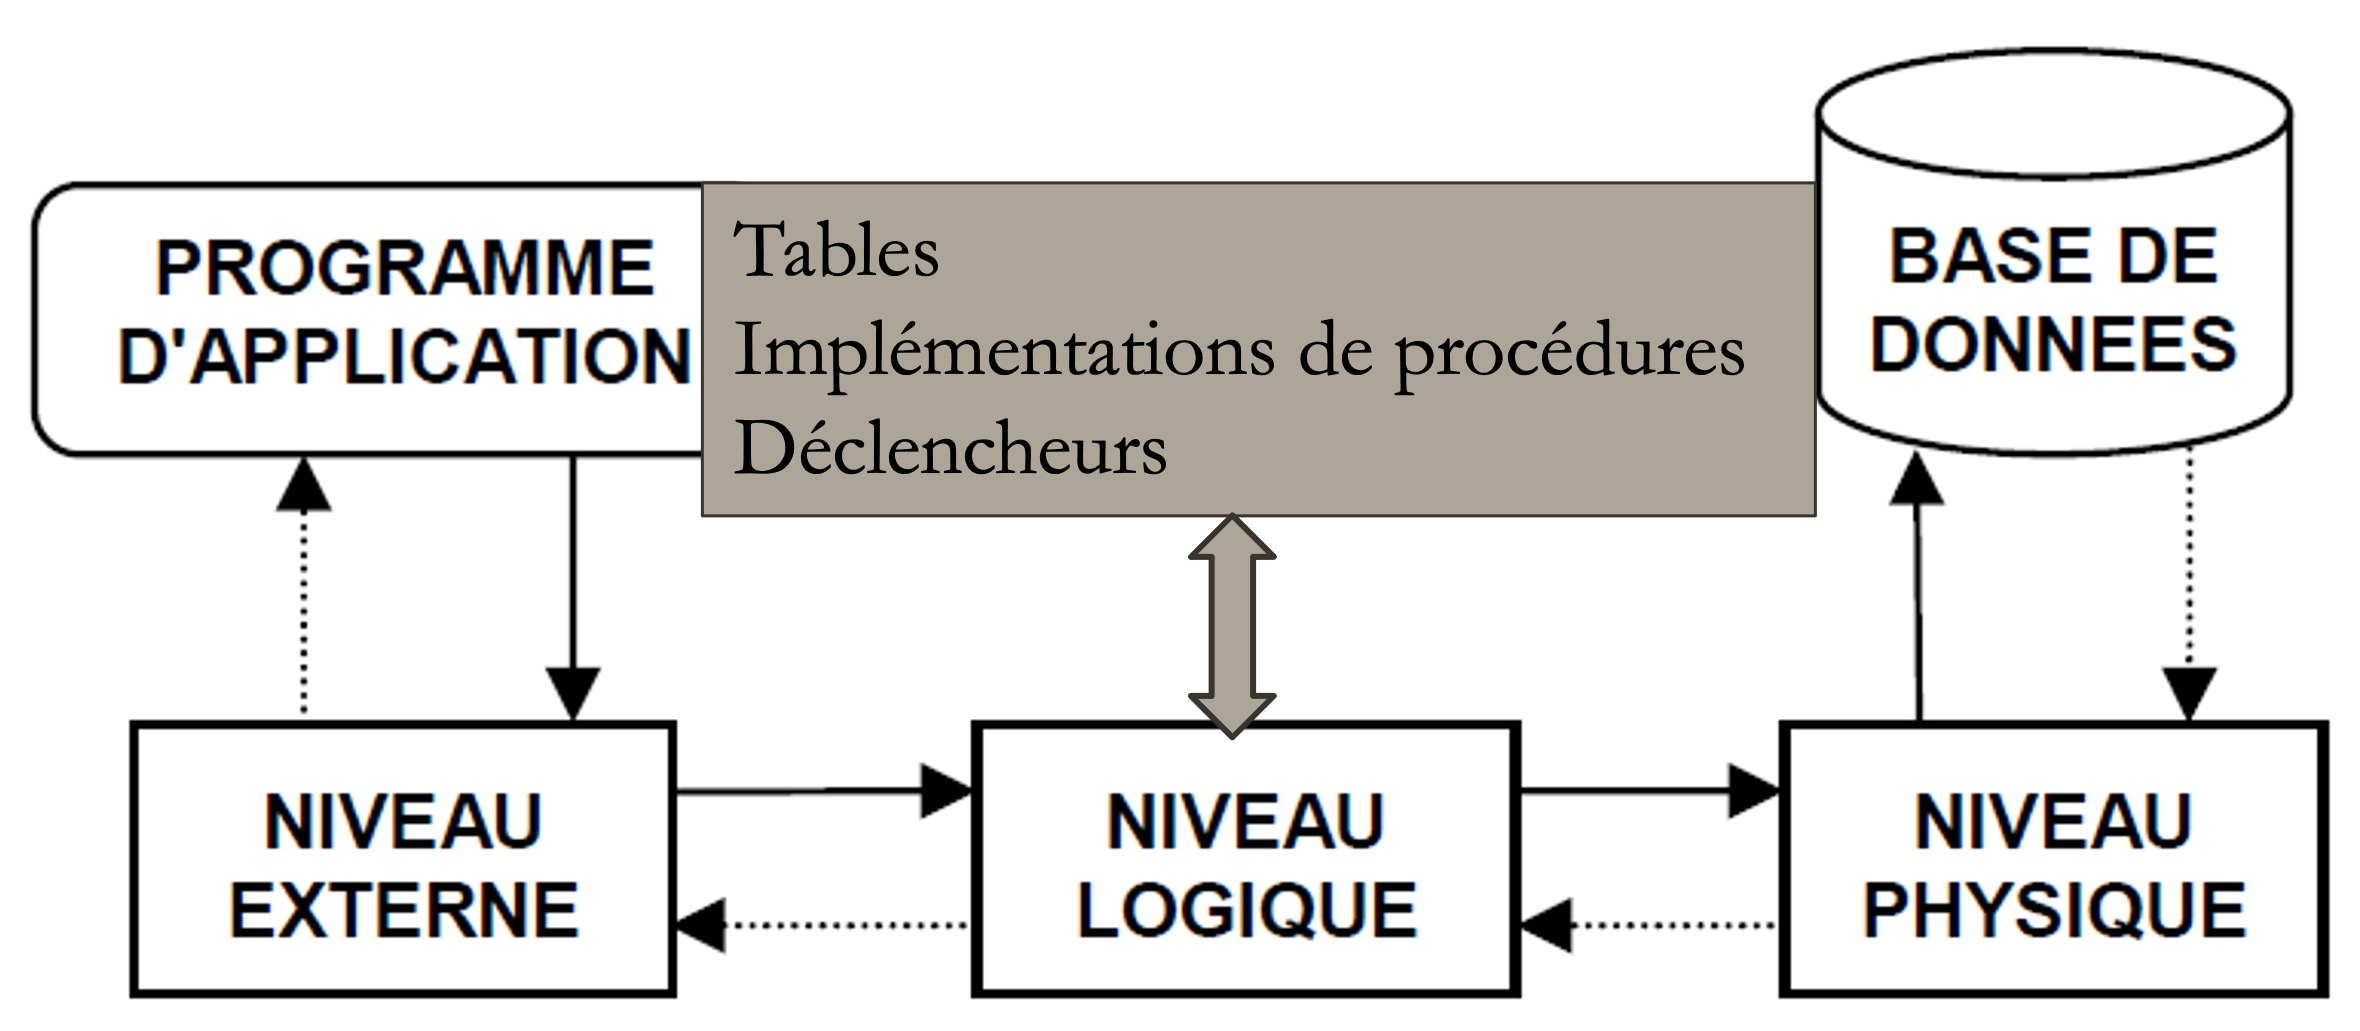
\includegraphics[width=0.55\textwidth]{../assets/img/par_sgbd_et_programme--2.jpg}
            \caption{Indépendance des données et des programmes}
            \label{Fig:par_sgbd_et_programme--2}
        \end{center}
    \end{figure}
\end{frame}

\begin{frame}{\subsecname : \subsubsecname}
    \begin{figure}
        \begin{center}
            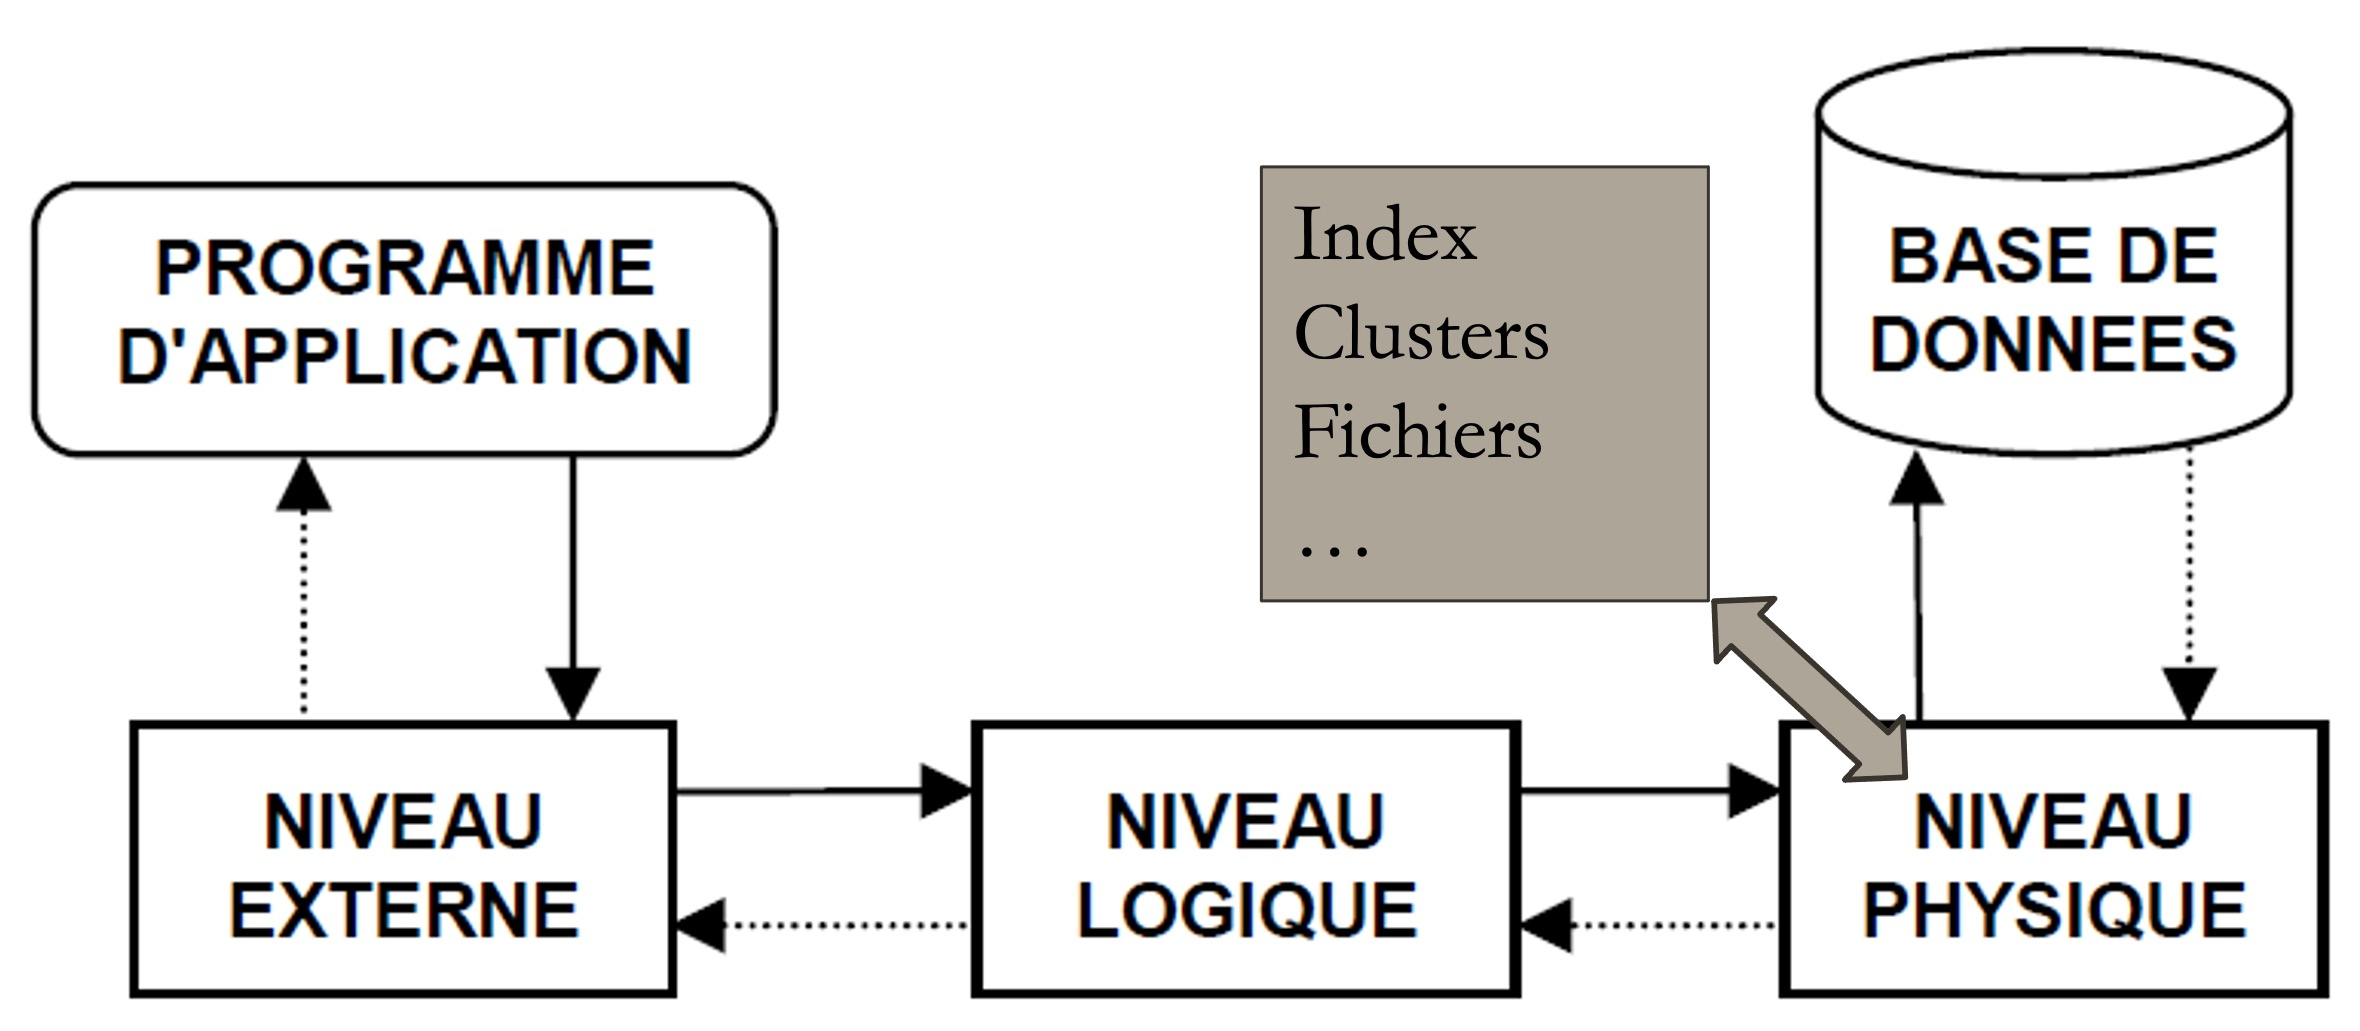
\includegraphics[width=0.55\textwidth]{../assets/img/par_sgbd_et_programme--3.jpg}
            \caption{Indépendance des données et des programmes}
            \label{Fig:par_sgbd_et_programme--3}
        \end{center}
    \end{figure}
\end{frame}
\begin{frame}{\subsecname : \subsubsecname}
    \begin{figure}
        \begin{center}
            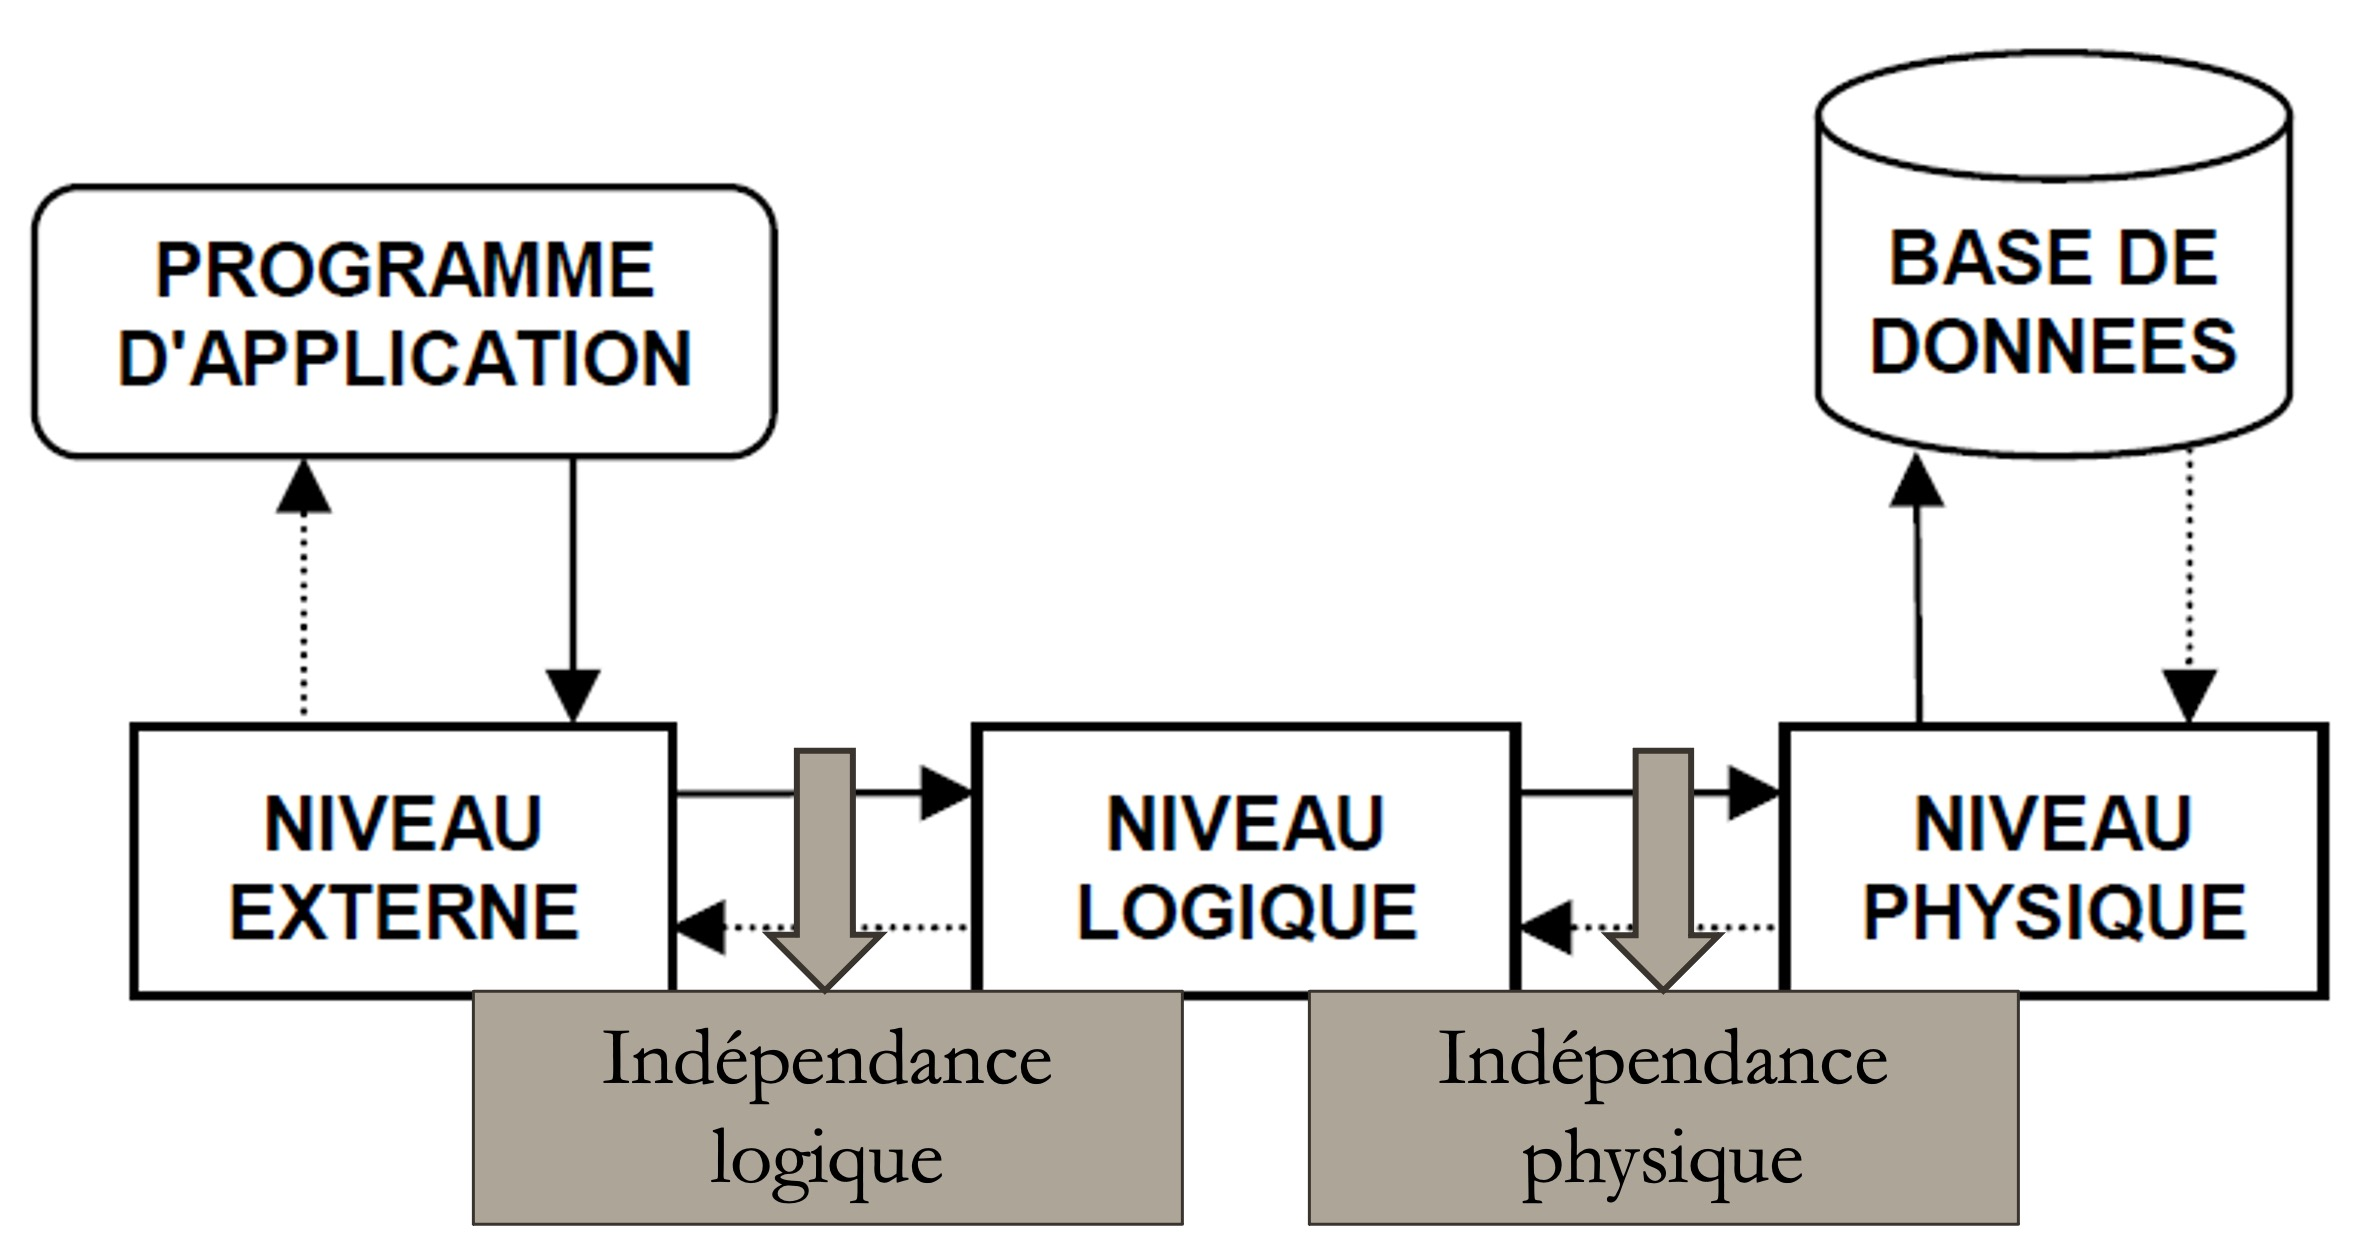
\includegraphics[width=0.55\textwidth]{../assets/img/par_sgbd_et_programme--4.jpg}
            \caption{Indépendance des données et des programmes}
            \label{Fig:par_sgbd_et_programme--4}
        \end{center}
    \end{figure}
\end{frame}

\begin{frame}{\subsecname : \subsubsecname}
    \begin{alertblock}{Important}
        \begin{itemize}
            \item L’\textbf{indépendance des données au niveau LOGIQUE} signifie que l’on peut changer la structure logique globale sans devoir changer les programmes d’applications.
            \item L’\textbf{indépendance des données au niveau PHYSIQUE} signifie que la couche physique et l’organisation des données peuvent changer sans devoir changer la structure logique globale ou les programmes d’applications.
        \end{itemize}
    \end{alertblock}
\end{frame}

\begin{frame}{\subsecname : \subsubsecname}
    \begin{table}[]
        \resizebox{\textwidth}{!}{%
            \begin{tabular}{|l|l|l|l|}
                \hline
                \multicolumn{1}{|c|}{\textbf{Pas de changement pour}}                            & \multicolumn{1}{c|}{\textbf{Pgm}} & \multicolumn{1}{c|}{\textbf{\begin{tabular}[c]{@{}c@{}}niv\\ log\end{tabular}}} & \multicolumn{1}{c|}{\textbf{\begin{tabular}[c]{@{}c@{}}Org\\ mém\end{tabular}}} \\ \hline
                Ajout d’1 nv pgm utilisant des données existantes                                & *                                 & *                                                        & *                                                        \\ \hline
                1 pgm utilise une nvelle représentation de données existantes                    & *                                 & *                                                        & *                                                        \\ \hline
                Ajout d’un nv pgm utilisant de nvelles données                                   & *                                 &                                                          &                                                          \\ \hline
                Description log glob améliorée / ajout nvelles assoc entre données               & *                                 &                                                          &                                                          \\ \hline
                Fusion de 2 BD                                                                   & *                                 & *                                                        &                                                          \\ \hline
                Organisation physique améliorée, éventuellement nvelle représentation de données & *                                 & *                                                        &                                                          \\ \hline
                Méthodes d’accès modifiées                                                       & *                                 & *                                                        &                                                          \\ \hline
                Données déplacées sur d’autres volumes                                           & *                                 & *                                                        &                                                          \\ \hline
                Logiciel est changé (nvelle version)                                             & *                                 & *                                                        &                                                          \\ \hline
                Matériel est changé                                                              & *                                 & *                                                        &                                                          \\ \hline
            \end{tabular}}
    \end{table}
\end{frame}
\section{Architecture d’un SGBD}
\subsection{Vue d'ensemble}
\begin{frame}{\secname : \subsecname}
    \begin{figure}
        \begin{center}
            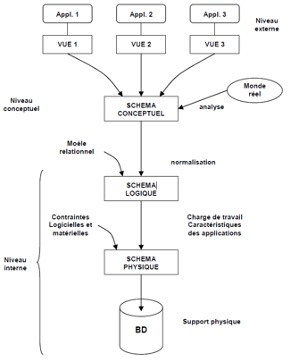
\includegraphics[width=0.35\textwidth]{../assets/img/architecture_sgbd--6.jpg}
            \caption{Vue d'ensemble}
            \label{Fig:architecture_sgbd--6}
        \end{center}
    \end{figure}
\end{frame}

\section{Avantages des bases de données}
\begin{frame}{\secname }
    \begin{itemize}
        \item La redondance peut être réduite (exception à la règle de non-redondance : pour améliorer vitesse de traitement et temps de réponse)
        \item L’incohérence peut être évitée
        \item Les données peuvent être partagées
        \item Des règles de sécurité peuvent être établies
        \item L’intégrité peut être maintenue
        \item Les conflits d’accès peuvent être équilibrés
    \end{itemize}
\end{frame}
\section{Fonctionnement d’un SGBD}
\begin{frame}{\secname }
    \begin{columns}
        \column{0.4\textwidth}
        Déroulement d’une recherche lancée par un programme d’application
        \column{0.6\textwidth}
        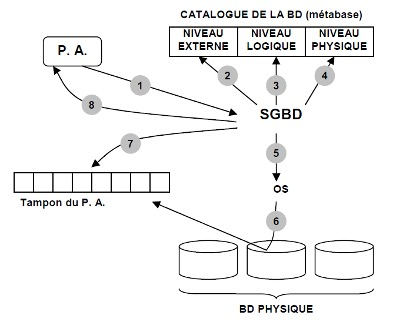
\includegraphics[width=0.8\linewidth]{../assets/img/architecture_sgbd--7.jpg}
    \end{columns}
\end{frame}


\end{document}
